\begin{lemma} \label{lemma:quadriertesummeinvarianzstrecken}
    Sei $s \subset \mathbb{R}^3$ eine Strecke, $\Omega$ einer der Symmetriegruppen $T$, $H$, $I$ und $\Pi_{E}:\mathbb{R}^3 \rightarrow E$ die orthogonale Projektion auf eine Ebene $E \subset \mathbb{R}^3$. Dann ist die Summe  
    \begin{align} \label{eq:sum_line_segment_projection_independent_of_plane}
        \sum_{w \in \Omega} \|\Pi_{E}w(s)\|^2  
    \end{align}
    unabhängig von $E$.
\end{lemma}

\begin{proof} 
Wir werden den Beweis nur für $\Omega = T$ zeigen, da wir einerseits noch einen Alternativbeweis zeigen und andererseits der Beweis analog für $\Omega \in \{H,I\}$ funktioniert. Sei $\Omega = T$. Wir wollen in diesem Beweis konkret nachrechnen, dass die Summe in Gleichung \eqref{eq:sum_line_segment_projection_independent_of_plane} konstant ist. Dafür müssen wir die Projektionen ausrechnen. Für die Orthogonalprojektion $\Pi_{E}$ gilt gemäss \eqref{eq:ortho_proj_matrix_notation}
\begin{align} 
    \Pi_{E}(\vec{v}) = (I - \vec{n}\vec{n}^T) \vec{v} = I - \begin{pmatrix}
        n_1^2 & n_1 n_2 & n_1 n_3 \\
        n_2 n_1 & n_2^2 & n_2 n_3 \\
        n_3 n_1 & n_3 n_2 & n_3^2
    \end{pmatrix}. \nonumber
\end{align}
Wie wir wissen, gilt $|T|=12$. Das bedeutet, wir müssen die $12$ Abbildungen ausrechnen. Dazu betrachten wir folgendes Tetraeder mit Kanten $(1,1,1)$, $(1,-1,-1)$, $(-1,1,-1)$ und $(-1,-1,1)$, siehe Abbildung \ref{fig:tetraederspezielleorientierung}.
\begin{figure}[htp]
    \centering
    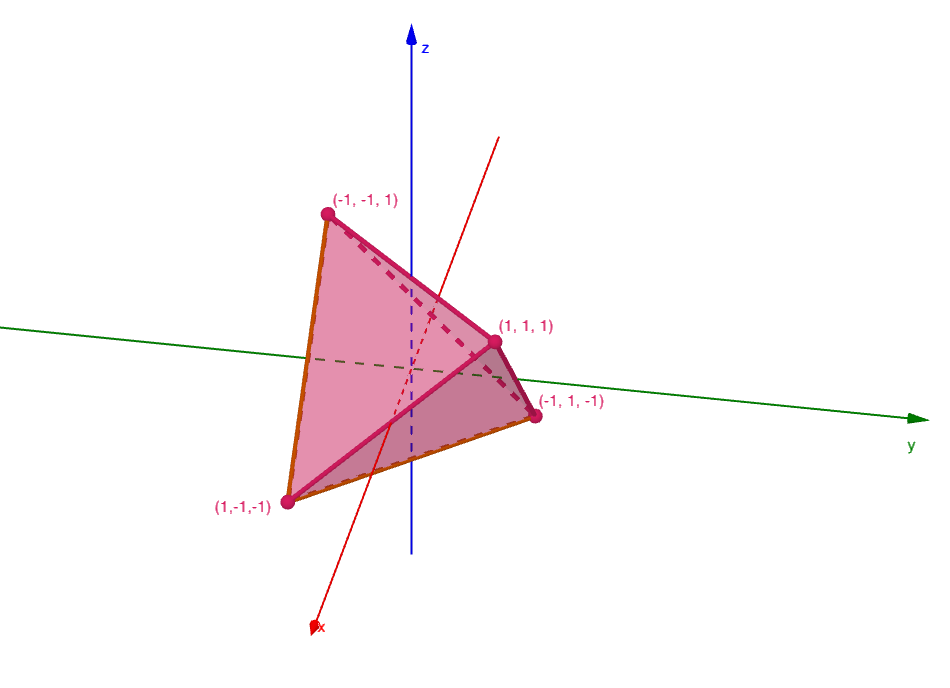
\includegraphics[width=0.6\textwidth]{images/polyeder/tetraederspeziellorientiert.png}
    \caption{Tetraeder mit Kanten $(1,1,1)$, $(1,-1,-1)$, $(-1,1,-1)$ und $(-1,-1,1)$.}
    \label{fig:tetraederspezielleorientierung}
\end{figure}
Wenn wir diese spezielle Ausrichtung des Tetraeders wählen, können wir die Rotationen um die Achsen von Typ $b$, siehe Abbildung \ref{fig:tetraederotationsachsen}, wie folgt darstellen:

\begin{align}
    A_0 = \begin{pmatrix} 1 & 0 & 0 \\ 0 & 1 & 0 \\ 0 & 0 & 1 \end{pmatrix}, \quad
    A_1 = \begin{pmatrix} 1 & 0 & 0 \\ 0 & -1 & 0 \\ 0 & 0 & -1 \end{pmatrix}, \nonumber \\
    A_2 = \begin{pmatrix} -1 & 0 & 0 \\ 0 & 1 & 0 \\ 0 & 0 & -1 \end{pmatrix}, \quad
    A_3 = \begin{pmatrix} -1 & 0 & 0 \\ 0 & -1 & 0 \\ 0 & 0 & 1 \end{pmatrix}. \nonumber
\end{align}
Die Rotation von Typ $a$ lässt sich mit der Matrix
\begin{align}
    R &= \begin{pmatrix} 0 & 0 & 1 \\ 1 & 0 & 0 \\ 0 & 1 & 0 \end{pmatrix} \nonumber
\end{align}
darstellen. Alle Abbildungen der Symmetriegruppe $T$ sind somit gegeben durch
$$ \left\{A_i R^k \mid k \in \{0,1,2\}, i \in \{0,1,2,3\} \right\}.$$
Somit können wir nun die Summe berechnen und wir erhalten
\begin{align}
    \sum_{w \in \Omega} \|\Pi_{E}w(s)\|^2  &= \sum_{k=0}^2 \sum_{i=0}^3 \|\Pi_{E}A_iR^k\|^2 \nonumber \\ 
    &=  \sum_{k=0}^2 \sum_{i=0}^3 \left\|\left(I - \begin{pmatrix}
        n_1^2 & n_1 n_2 & n_1 n_3 \\
        n_2 n_1 & n_2^2 & n_2 n_3 \\
        n_3 n_1 & n_3 n_2 & n_3^2
    \end{pmatrix}\right)A_iR^k\vec{s} \ \right\|^2  \nonumber \\
    &=8 \|\vec{s}\|^2, \nonumber
\end{align}
wobei wir die Tatsache benutzt haben, dass die Strecke $s$ unter Translation ihre Länge nicht verändert. Inbesondere, dass wir die Strecke $s$ auf den Ursprung verschieben können und dementsprechend $s$ als Vektor $\vec{s} \in \mathbb{R}^3$ betrachten können. 
\end{proof}
Wir möchten hier anmerken, dass das Ausmultiplizieren der Matrizen im Beweis keine schwierige, jedoch eine zeitintensive Aufgabe ist. Wir ermutigen die LeserInnen zumindest einmal die Rechnung selbst per Hand auszurechnen. Wie schon im Beweis erwähnt, folgen die Beweise für $\Omega \in \{H,I\}$ demselben Schema. Da die Kardinalität der Symmetriegruppen jedoch grösser ist, wird der Rechenaufwand dementsprechend auch grösser. Da kommt es gerade gelegen, dass wir anstatt die Summe der Kantenlängen unter der Orthogonalprojektion, siehe Gleichung \eqref{eq:sum_projection_independent_of_plane}, direkt auszurechnen, auch über die Irreduzibilität von den Symmetriegruppen den Beweis führen können.
\begin{proof}
    Sei $\vec{s} \in \mathbb{R}^3$ der Richtungsvektor der Strecke $s$. Wir nutzen die Zerlegung aus Gleichung \eqref{eq:vektor_parallel_senkrecht} und die Darstellung der Projektionslänge aus \eqref{eq:projectionwithvectorandnormal}. Für ein beliebiges $w \in \Omega$ gilt:
    \begin{align} 
        \|\Pi_{E}w(\vec{s})\|^2 &= \|w_{\parallel}(\vec{s})\|^2 \nonumber \\
        &= \|w(\vec{s})\|^2 - \|w(\vec{s})_{\perp}\|^2 \nonumber \\
        &= \|w(\vec{s})\|^2 - \|\left(\vec{n}_E \cdot w(\vec{s})\right)\vec{n}_E\|^2, \nonumber
    \end{align}
    wobei $\vec{n}_E$ der Normalenvektor der Ebene $E$ ist, d.h. $\|\vec{n}_E\| = 1$. Da alle Abbildungen $w \in \Omega$ Drehungen und somit Isometrien (längenerhaltend) sind, gilt $\|w(\vec{s})\|^2 = \|\vec{s}\|^2$. Summiert über die gesamte Gruppe ergibt sich:
    \begin{align} 
        \sum_{w \in \Omega} \|\Pi_{E}w(\vec{s})\|^2 &= \sum_{w \in \Omega} \left( \|w(\vec{s})\|^2 - \|\left(\vec{n}_E \cdot w(\vec{s})\right)\vec{n}_E\|^2 \right) \nonumber \\
        &= \sum_{w \in \Omega} \left( \|\vec{s}\|^2 - |\vec{n}_E \cdot w(\vec{s})|^2 \|\vec{n}_E \|^2\right) \nonumber \\
        &= |\Omega|  \|\vec{s}\|^2 - \sum_{w \in \Omega} |\vec{n}_E \cdot w(\vec{s})|^2. \nonumber
    \end{align}
    Der erste Term $|\Omega| \cdot \|\vec{s}\|^2$ ist konstant. Um die Unabhängigkeit bezüglich der Ebene $E$ zu zeigen, müssen wir nachweisen, dass auch der zweite Term konstant ist. Unter Verwendung der Identität $(\vec{a} \cdot \vec{b})^2 = \vec{a}^T(\vec{b} \ \vec{b}^T)\vec{a}$ erhalten wir:
    \begin{align} \label{eq:summevectormatrixnormal_revised}
        \sum_{w \in \Omega} |\vec{n}_E \cdot w(\vec{s})|^2 &= \sum_{w \in \Omega} \vec{n}_E^T \left( w(\vec{s}) w(\vec{s})^T \right) \vec{n}_E \nonumber \\
        &= \vec{n}_E^T \left( \sum_{w \in \Omega} w(\vec{s}) w(\vec{s})^T \right) \vec{n}_E.
    \end{align}
    Wir definieren die Matrix $$M := \sum_{w \in \Omega} w(\vec{s}) w(\vec{s})^T \in \mathbb{R}^{3 \times 3}.$$ 
        Das bedeutet, unsere Summe aus Gleichung \eqref{eq:sum_line_segment_projection_independent_of_plane} lässt sich wie folgt schreiben
       \begin{align} \label{eq:summemitmatrixM}
        \sum_{w \in \Omega} \|\Pi_{E}w(\vec{s})\|^2 = |\Omega|  \|\vec{s}\|^2 - \vec{n}_E^T M \vec{n}_E.
    \end{align}
    Nun stellt sich uns die Frage, wann der hintere Term konstant ist. Zuerst tragen wir jedoch zusammen, welche Eigenschaften die Matrix $M$ hat:
    \begin{itemize}
        \item[I.]  Die Matrix $M$ ist symmetrisch ($M=M^T$). Gemäss dem Spektralsatz, siehe Anhang \ref{sec:spektralsatzlinearealgebra}, besitzt die symmetrische Matrix $M$ einen reellen Eigenwert $\lambda$ mit zugehörigem Eigenraum $V_\lambda \neq \{0\}$.
        \item[II.] Die Matrix $M$ kommutiert mit jeder Drehung $R \in \Omega$:
    \begin{align}
        R M R^T &= \sum_{w \in \Omega} R w(\vec{s}) w(\vec{s})^T R^T = \sum_{w \in \Omega} (R w(\vec{s})) (R w(\vec{s}))^T= M, \nonumber
    \end{align}
 da die Multiplikation mit $R$ von links die Gruppenelemente lediglich permutiert. Wie wir bereits in Abschnitt \ref{sec:orthogonalrotation} gesehen haben, sind Drehungen orthogonal und es folgt 
 \begin{align} 
    RM = MR. \nonumber
 \end{align}
    \end{itemize}

 Für einen Vektor $\vec{v} \in V_\lambda$ gilt somit
    \begin{align}
        M(R\vec{v}) \overset{II.}{=} R(M\vec{v}) \overset{I.}{=} R(\lambda \vec{v}) = \lambda (R\vec{v}). \nonumber
    \end{align}
    Somit ist $R\vec{v} \in V_\lambda$, was bedeutet, dass $V_\lambda$ ein invarianter Unterraum unter der Wirkung von $\Omega$ ist. Da die Gruppen $T, H$ und $I$ nach Lemma \ref{lemma:irreduzibelsymmetriegruppen} irreduzibel auf dem $\mathbb{R}^3$ operieren, muss $V_\lambda = \mathbb{R}^3$ gelten. Daraus folgt, dass $M$ ein skalares Vielfaches der Einheitsmatrix ist: $$M = \lambda I_3.$$
    
    Eingesetzt in Gleichung \eqref{eq:summevectormatrixnormal_revised} ergibt sich:
    \begin{align}
        \sum_{w \in \Omega} |\vec{n}_E \cdot w(s)|^2 = \vec{n}_E^T (\lambda I_3) \vec{n}_E = \lambda (\vec{n}_E^T \vec{n}_E) = \lambda. \nonumber
    \end{align}
    Da $\lambda$ eine Konstante ist, ist die Summe der quadrierten Projektionslängen unabhängig von der Ebene $E$.
\end{proof}



